\documentclass[11pt]{article}
\usepackage{amsfonts}
\usepackage{amsmath}
\usepackage{amsthm}
\usepackage{amssymb}
\usepackage{mathrsfs}
\usepackage[fit]{truncate}
\usepackage{acl2012}
\usepackage{times}
\usepackage{latexsym}
\usepackage{amsmath}
\usepackage{url}
\usepackage{graphicx}
%\usepackage{caption}
\usepackage[font=small]{caption}
\usepackage{multirow}
\usepackage{dblfloatfix}
\usepackage{float}
\usepackage{subfloat}
\usepackage{subcaption}

\setlength\titlebox{5cm}    % Expanding the titlebox
\setlength{\abovecaptionskip}{1pt plus 1pt minus 1pt} % Chosen fairly arbitrarily
\setlength{\belowcaptionskip}{1pt plus 1pt minus 1pt} % Chosen fairly arbitrarily

\newcommand{\affliationPenn}{\ensuremath{{}^\text{1}}}
\newcommand{\affliationJHU}{\ensuremath{{}^\text{2}}}

\title{The Language Demographics of  Amazon Mechanical Turk : Response  to Reviewers}

\author{Ellie Pavlick\affliationPenn \ \ \ \ \ Ann Irvine\affliationJHU  \ \ \ \ \ Dmitry Kachaev\affliationJHU  \ \ \ \ \  Chris Callison-Burch\affliationPenn$^{,}$\affliationJHU \\
\affliationPenn Computer and Information Science Department, University of Pennsylvania \\
\affliationJHU Human Language Technology Center of Excellence, Johns Hopkins University \\
  }
  
% Anonymized for submission
\author{}

\date{}

\begin{document}
\maketitle

%\begin{figure}
%\centering
%\begin{subfigure}[b]{1\linewidth}
%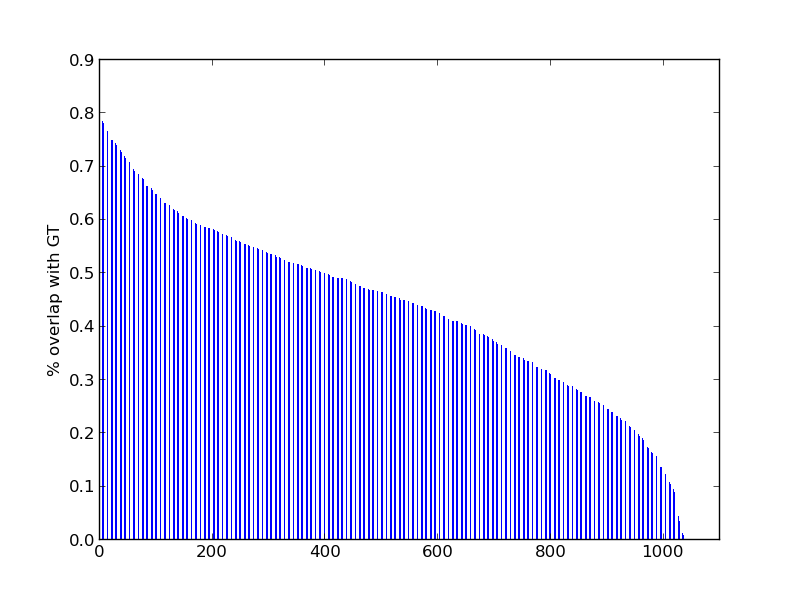
\includegraphics[width=\textwidth]{figures/turker-googmatch-distribution.png}
%\caption{Individual turker overlap with Google Translate. We remove the 500 workers with the highest overlap (shaded region on the left) from our analysis, as it is reasonable to assume these workers are cheating by submitting translations from Google. We believe the workers with no overlap (shaded region on the right) are also likely to be cheating, e.g. by submitting random text, and we target these workers through our embedded quality controls.}                
%\label{dist}
%\end{subfigure}
%\begin{subfigure}[b]{1\linewidth}
%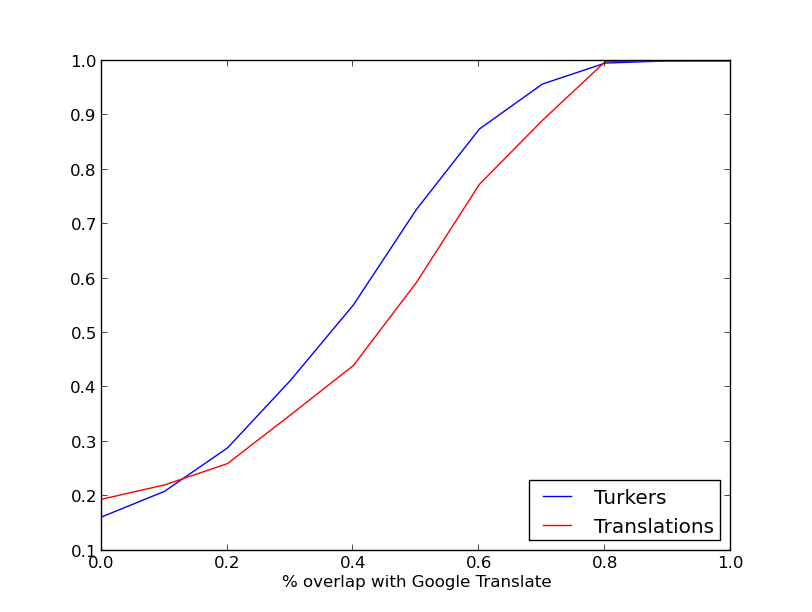
\includegraphics[width=\textwidth]{figures/google-cdf-googlangs.png}
%\caption{Cumulative distribution of overlap with Google translate for workers and translations. We see that eliminating all workers with \textgreater 70\% overlap with google translate still preserves 90\% of translations and \textgreater 90\% of workers.}
%\label{cdf}
%\end{subfigure}
%\caption{}\label{cheaters}
%\end{figure}

\section{Use of Google Translate : Editor and all reviewers}

The primary concern across reviewers was the high amount of overlap between workers' translations and translations available through online resources, i.e. Google Translate. The editor summarized : 
\begin{quote}
All reviewers had issues with the amount of cheating taking place among Turkers. It would be useful to quantify/detect this and remove such participants from your results.
\end{quote}

\begin{figure}[ht]
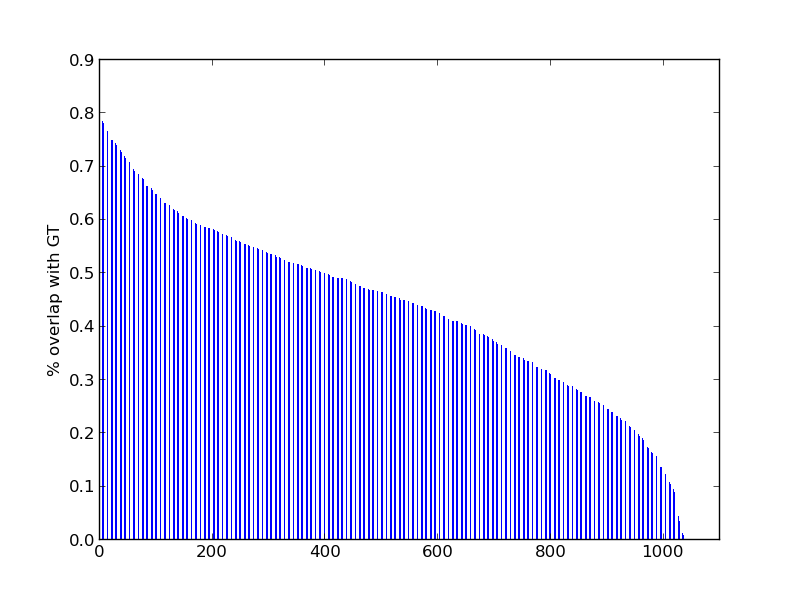
\includegraphics[width=\linewidth]{figures/turker-googmatch-distribution.png}
\caption{Individual turker overlap with Google Translate. We remove the 500 workers with the highest overlap (shaded region on left) from our analysis. Workers with no overlap (on right) are also likely to be cheating, e.g. by submitting random text. We target these workers through our embedded controls.}                
\label{dist}
\end{figure}

\begin{figure}[h]
\centering
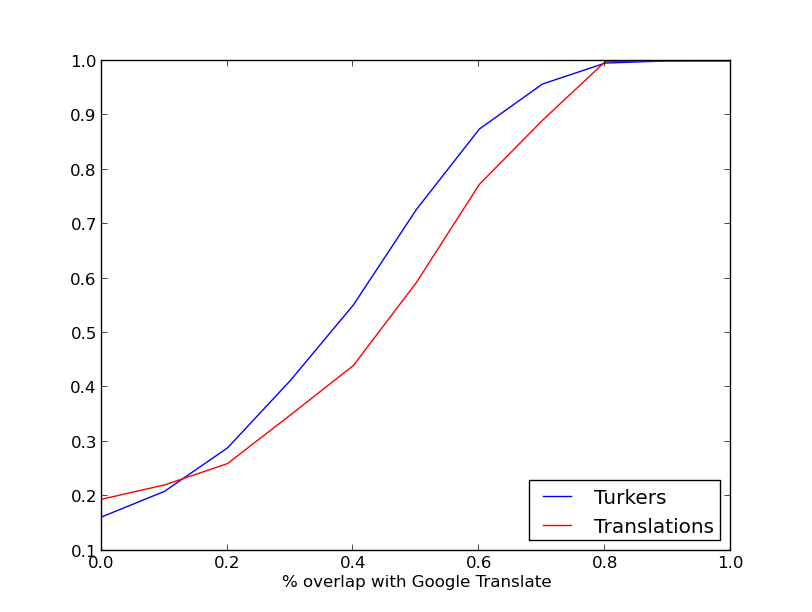
\includegraphics[width=\linewidth]{figures/google-cdf-googlangs.png}
\caption{Cumulative distribution of overlap with Google translate for workers and translations. Eliminating all workers with \textgreater 70\% overlap with google translate still preserves 90\% of translations and \textgreater 90\% of workers.}
\label{cdf}
\end{figure}

We took at closer look at the amount of overlap with Google translate in our collected translations in order to address this issue. We found that while overall overlap is high, it is not consistantly high across all turkers. Figure \ref{dist} shows that while a small number of turkers have a very high amount of overlap with Google (near 80\%) the majority overlap less than half of the time. 

%As Reviewer E noted : 

%\begin{quote}
%..it is quite possible that a fluent speaker of a language provides the same translation as Google Translate for a given word.  In other words, the performance results are inconclusive.
%\end{quote}



It seems likely that those with very high overlap are cheating, but it is also reasonable to assume that honest turkers will overlap with Google with some regularity. We therefore divide the workers into three groups : those with very high overlap with Google (likely cheating by using Google to translate words), those with reasonable overlap, and those with no overlap (likely cheating by other means, e.g. submitting random text). Our controls are designed to identify workers that fall into the third group (those who are spamming or providing useless translations), but they will not effectively flag workers who are cheating with Google Translate. 



We chose to remove the 500 turkers with the highest overlap with Google. This equates to removing all workers with greater than 70\% overlap. Figure \ref{cdf} shows that removing workers at or above the 70\% threshold retains 90\% of the collected translations and over 90\% of the workers.

\begin{figure}
\centering
\begin{subfigure}[b]{1\linewidth}
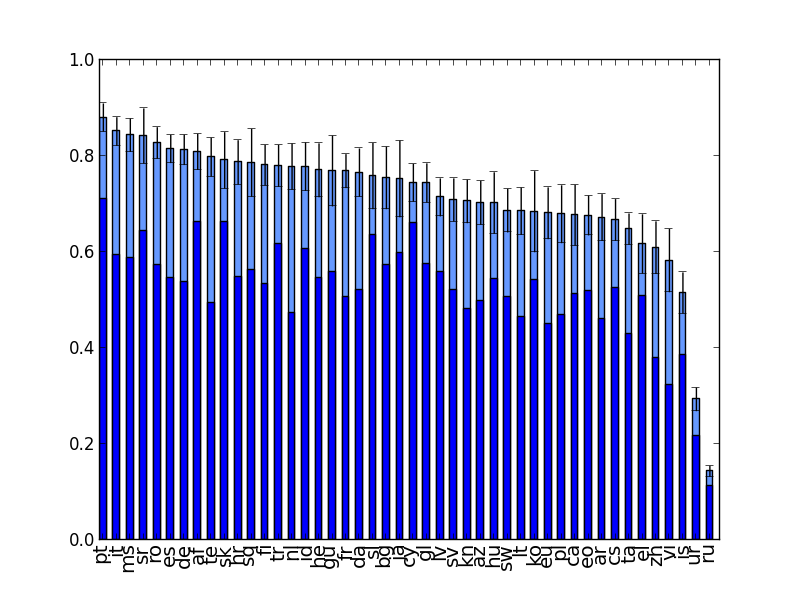
\includegraphics[width=\textwidth]{figures/quality-all.png}
\caption{All turkers.}                
\label{quality-all}
\end{subfigure}
\begin{subfigure}[b]{1\linewidth}
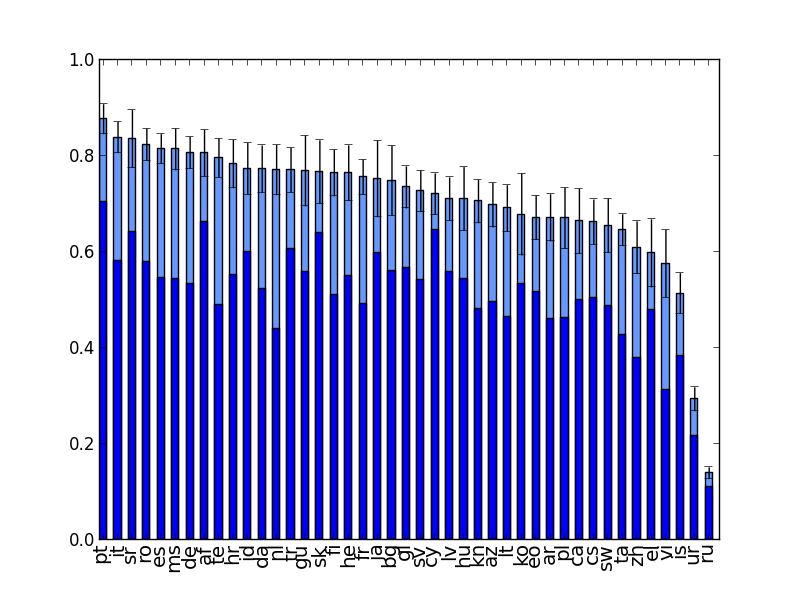
\includegraphics[width=\textwidth]{figures/quality-filtered.png}
\caption{Turkers with \textless 70\% overlap with Google Translate.}
\label{quality-filtered}
\end{subfigure}
\caption{Qualities for languages with \textgreater 50 turkers. Dark blue shows quality measured by perfect match on the control translation. Light blue indicates quality measured by included synonymous translations.}\label{qual}
\end{figure}

We have rerun the quality analysis in the paper, omitting workers with \textgreater 70\% overlap with Google Translate. The quality scores and rankings do not change substantially. For reference, figure \ref{qual} shows the quality scores for languages when computed over all Turkers as in the original draft of the paper (figure \ref{quality-all}) and computed over only Turkers with less than 70\% overlap with Google (figure \ref{quality-filtered}). In our new draft of the paper, we have omitted Tukers with more than 70\% overlap from all of our quality computations.


%\begin{figure}
%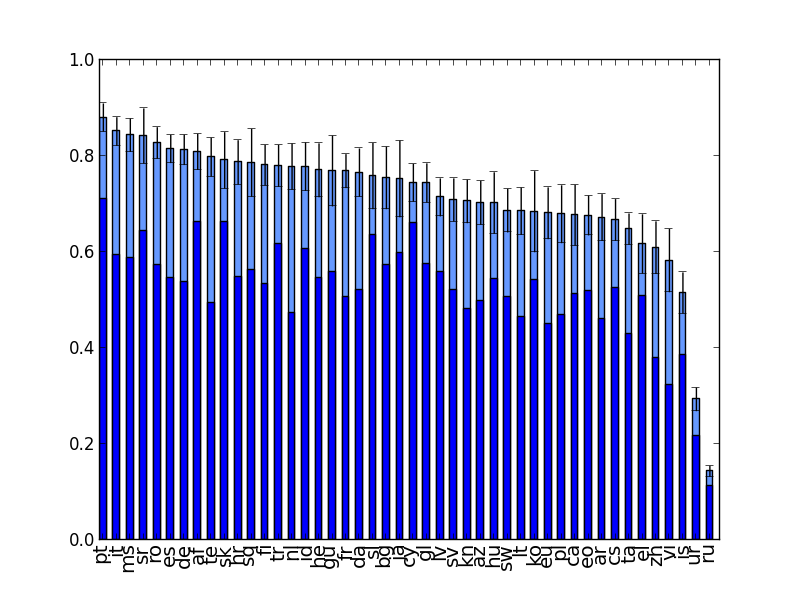
\includegraphics[width=\linewidth]{figures/quality-all.png}
%\caption{All turkers.}                
%\label{quality-all}
%\end{figure}
%\begin{figure}
%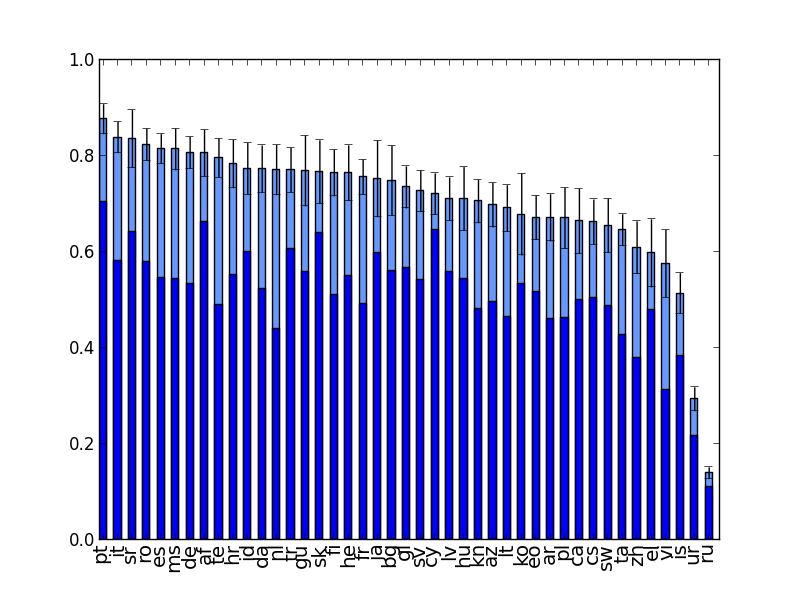
\includegraphics[width=\linewidth]{figures/quality-filtered.png}
%\caption{Turkers with \textless 70\% overlap with Google Translate.}
%\label{quality-filtered}
%\caption{Qualities for languages with \textgreater 50 turkers. Dark blue shows quality measured by perfect match on the control translation. Light blue indicates quality measured by included synonymous translations.}\label{qual}
%\end{figure}


\section{Robustness of results to removing few big players: Editor and all reviewers}

The editor and reviewer G highlighted the possibility that the quality results are due to a few large players, and may not be robust if the experiment were rerun with a different group of workers : 
\begin{quote}
Provide additional analysis showing that translation accuracy is not due to a few individuals who happened to do most of your tasks.
\end{quote}

We agree that this is a valid concern since many languages followed the pattern of having a small number of very active Turkers complete the majority of assignments. We account of this by reporting qualities of each language as an average over Turker qualities, rather than over assignment qualities. By this method, each Turker contributes equally to the language's average quality, regardless of the number of HITs that that Turker submitted. Section 4 of the paper has been updated to reflect this change. Figure \ref{qual_dots} shows the quality scores for languages computed over assignments and over Turkers, and the change in each when the 10 most active Turkers in each language are removed. We can see that the per-Turker quality measure is robust to the exclusion of these highly-contributing Turkers. 

For completeness, we have also updated our reported quality scores in the paper to include confidence intervals and p-values, where appropriate. We hope this helps to reduce concern about the robustness of these measures.

%\begin{figure}
%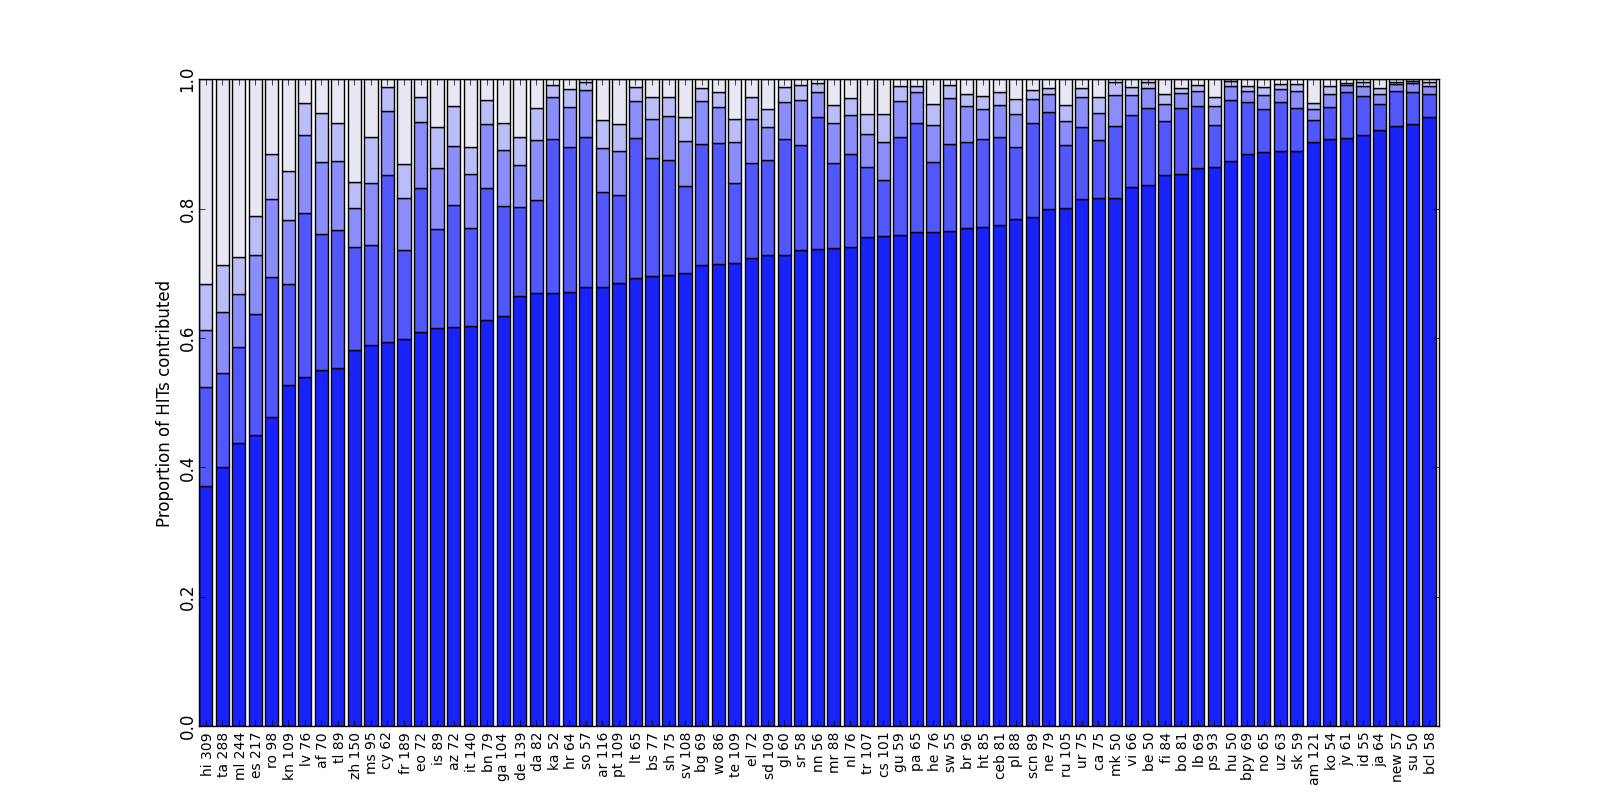
\includegraphics[height=1\linewidth, angle=270]{figures/turker-hit-contributions.png}
%\caption{Contributions of individual turkers to the overall number of HITs in each language. The dark blue bar represents the proportion of total HITs which were completed by the 10 highest-contributing turkers. The next darkest bar represents the next 10 highest-contributing turkers, and likewise for the thrid and forth darkest. The final bar represents the remaining turkers which were not one of the top 40 contributors.}
%\label{num./hits}
%\end{figure}

\begin{figure}
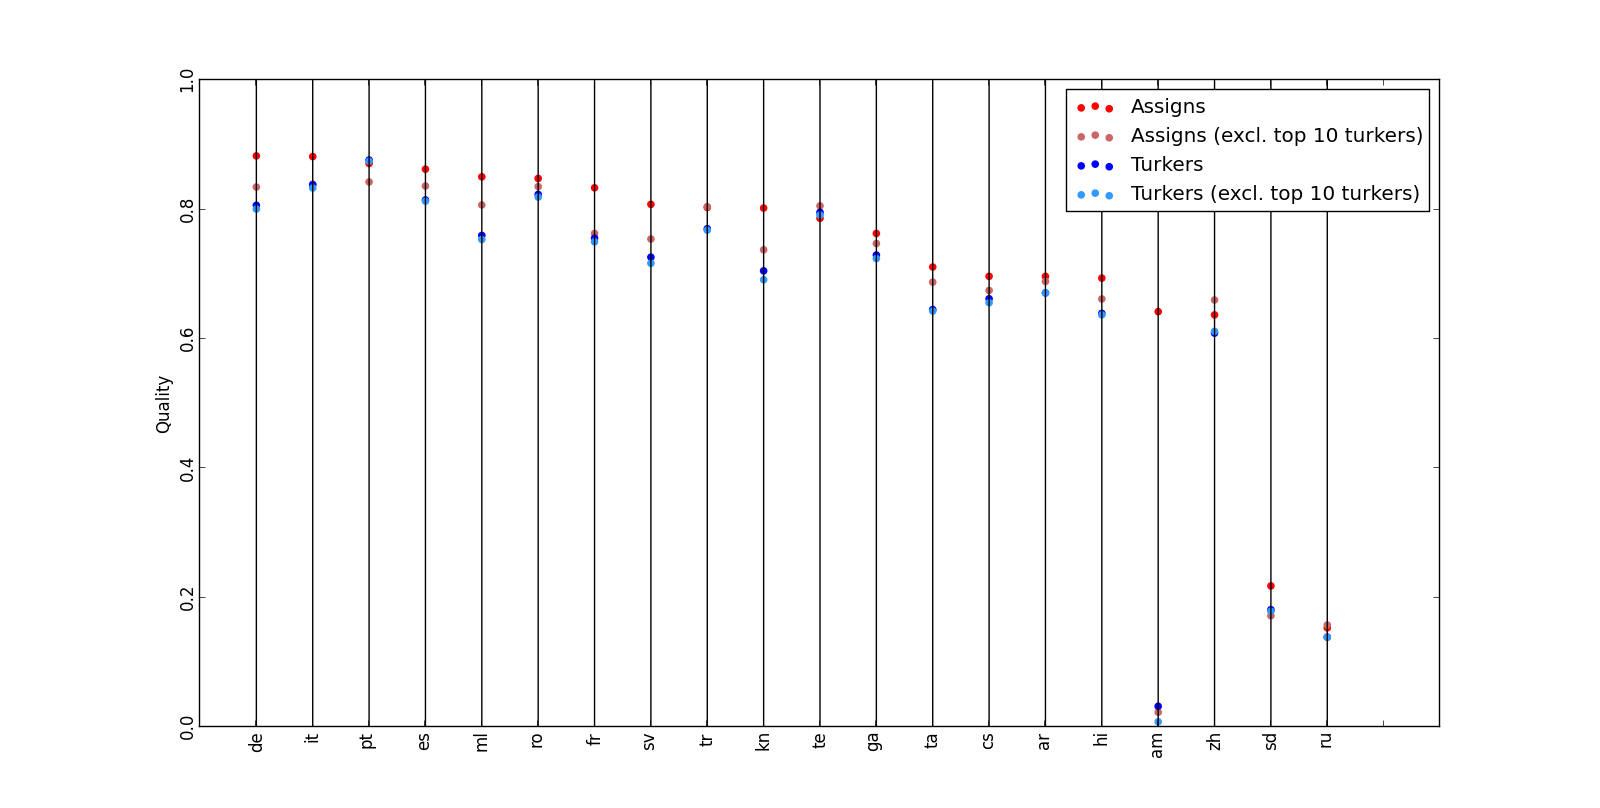
\includegraphics[height=1\linewidth, angle=270]{figures/quality_compare.png}
\caption{Quality scores of languages computed as averages over assignments (red) and over turkers (blue). Light blue and light red dots reflect the quality scores that result when the 10 turkers with who contributed the highest number of HITs are removed. We see that while the quality calculated over assignments responds noticeably to the exclusion of these highly active turkers, the quality calculated over turkers is quite robust to the change.}
\label{qual_dots}
\end{figure}

\section{Extrinsic evalutation of mturk data for SMT: Editor and all reviewers}

All the reviewers expressed desire for further evidence of the usefulness of the Turker-provided translations for statistical machine translation, and the possibility of extending the demonstrated methods to multiple word translations. The editor requests :

\begin{quote}
It would be interesting to show that the proposed approach brings an advantage over current SMT technology, i.e., improves lexical translations for an existing SMT system....It would also be interesting to assess whether your results carry over to multiple words and/or sentences. 
\end{quote}

To address these concerns, we incorporate previous work from a workshop publication from our colleague. The workshop publication will be cited appropriately in the final version of the paper, but we omit the citation now so as not to de-anonymize the submission. 

In this work, we collect full-sentence translations for six Indian languages which are well-represented on MTurk but for which there are currently no professionally-translated corpora available. We use the collected sentences to train and evaluate an SMT system, and show that the systems achieve decent performance. Furthermore, we add the collected single-word dictionaries to the training of these systems, and show that this produces measurable improvement in performance. Table \ref{dictionary_bleu} highlights these results. Please see sections 3 and 5 for a complete discussion of the data and experiments. 

\begin{table}[t]
\centering
\begin{tabular}{l|ccc}
  language  & sentences &  dictionaries & Google \\
  \hline\hline
  Bengali    &  12.03 & 17.29 & 20.01 \\
  Hindi      & 16.19 & 18.10 & 25.21\\  
  Malayalam    &  6.65 & 9.72 & - \\      
  Tamil      & 8.08 & 9.66 & 13.51\\  
  Telugu     & 11.94 & 13.70 & 16.03\\  
  Urdu        & 19.22 & 21.98 & 23.09\\   
\end{tabular}
\caption{BLEU scores for translating into English using full sentence translations alone, and with the addition of single-word dictionaries. Scores are calculated using four reference translations and represent the mean of three MERT runs.}
\label{dictionary_bleu}
\end{table}

\section{Affect of time of day when HIT was posted: Reviewer F}

You raised an interesting question about the affect of time of day on Turker activity : 

\begin{quote}
Did the authors take into account time of day, when the HIT was posted etc. to get a sense of whether one time of day is more optimal than others for each language? Does it matter at all?
\end{quote}
Figure \ref{time} shows the activity over a 24 hour day for 23 languages with greater than 100 turkers each. The plot shows that activity does vary across time zones, and suggests that choosing the release time intelligently based on the HIT language is likely to affect how quickly it is completed. We include this analysis here for the interest of the reviewer. We do not include it in the paper, however, as we do not feel it meaningfully changes the analysis presented there. 

\begin{figure}
\centering
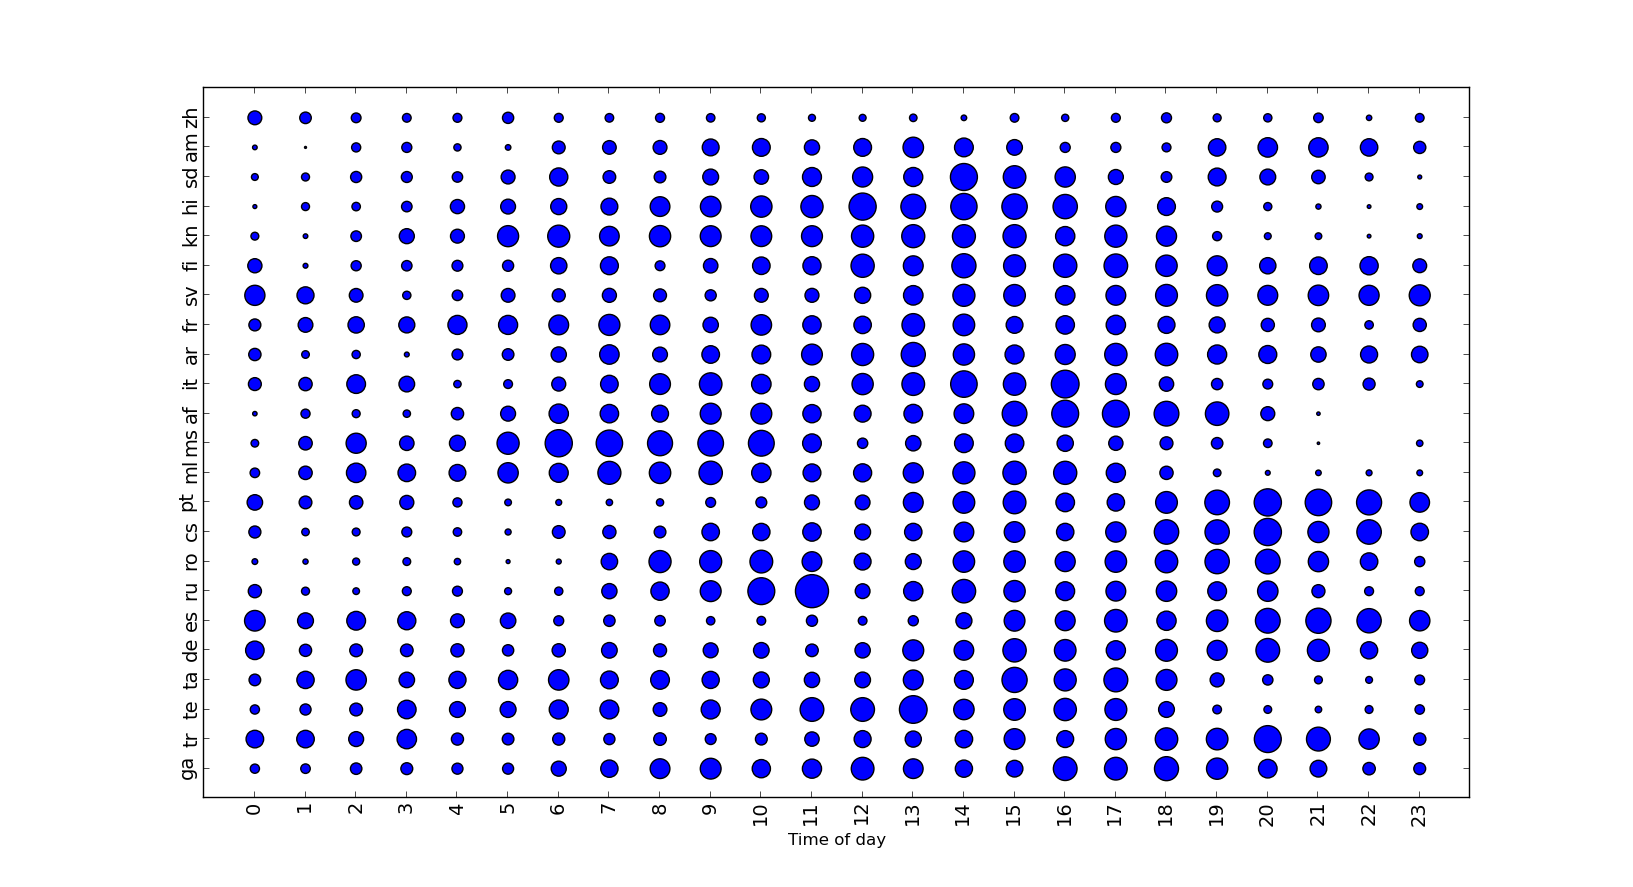
\includegraphics[height=.8\linewidth, angle=270]{figures/times.png}
\caption{Number of HITs completed during each hour of the day for languages with \textgreater 100 turkers.}
\label{time}
\end{figure}

\section{Changes in results if study continued over time: Reviewer B}

You asked : 
\begin{quote}
The authors ran an experiment over 3.5 months, but I wonder how the demographics change over time. Are there seasonal effects in the workforce? Has it changed over the past year? And more importantly, will it change substantially in the future? I'm somewhat skeptical that these demographics will remain constant, especially as Amazon rolls out changes to the service.
\end{quote}

While we agree that the questions posed are very interesting, we feel that answering these questions is the subject of another study. It is true that the current demongraphic makeup of MTurk workers is likely to shift, but we cannot currently take on the expense of conducting a long term study (the study presented here cost ~40K). We have updated the text of the paper to emphasize this limitation in our results by adding the following sentences to our Overview: 
\begin{quote}
While the demographics reported are likely to shift overtime, as Amazon expands its methods of payments and reaches new countries, the data presented provides a 
valuable snapshot of the current state of MTurk, and the methods used can be applied generally in future research.
\end{quote}

\section{Accuracy of Geolocation: Reviewers B and E}

We understand that geolocation is not perfect, which is why we propose the use of location data as just one of several criteria by which to identify likely qualified translators. The trends that we observe in our analysis, where we show that turkers geolocated within a region likely to speak the source language being translated tend to perform better on our controls, coincide with what we would expect to see if geolcation were accurate. Additionally, of the turkers who responded to our survey questions, 95\% of their self-reported locations agreed with our geolocations. These facts reassure us that, on average, the geolocation is performing sufficiently well.

\end{document}
